\documentclass[12pt]{article}

\usepackage{float}

\usepackage{standalone}

\usepackage[utf8x]{inputenc}

%%% PAGE DIMENSIONS
\usepackage{geometry}
\geometry{a4paper}
\geometry{margin=2.54cm} % for example, change the margins to 2 inches all round

\usepackage{graphicx} % support the \includegraphics command and options

\usepackage[parfill]{parskip} % Activate to begin paragraphs with an empty line rather than an indent

%%% PACKAGES
\usepackage{booktabs} % for much better looking tables
\usepackage{array} % for better arrays (eg matrices) in maths
\usepackage{paralist} % very flexible & customisable lists (eg. enumerate/itemize, etc.)
\usepackage{verbatim} % adds environment for commenting out blocks of text & for better verbatim
\usepackage{subfig} % make it possible to include more than one captioned figure/table in a single float
% These packages are all incorporated in the memoir class to one degree or another...

\usepackage{multicol}
\usepackage{multirow}
\usepackage{xcolor}
\usepackage{amsmath}

\usepackage[T1]{fontenc}
\usepackage{lmodern}

\usepackage{makecell}

\renewcommand{\arraystretch}{1.1}

%%% HEADERS & FOOTERS
\usepackage{fancyhdr} % This should be set AFTER setting up the page geometry
\pagestyle{fancy} % options: empty , plain , fancy
\fancyhead[L]{\leftmark}
\fancyhead[C]{}
\fancyhead[R]{\rightmark}
\fancyfoot[L]{}
\fancyfoot[C]{}
\fancyfoot[R]{\thepage}
\renewcommand{\headrulewidth}{0pt}
\renewcommand{\footrulewidth}{0pt}

\fancypagestyle{plain}{
	\fancyhf{} % clear all header and footer fields
	\fancyfoot[R]{\thepage} % except the center
	\renewcommand{\headrulewidth}{0pt}
	\renewcommand{\footrulewidth}{0pt}
}

%%% BIBILIOGRAPHY
\usepackage[numbers]{natbib}
\bibliographystyle{vancouver}

%%% SECTION TITLE APPEARANCE
\usepackage{sectsty}
\allsectionsfont{\sffamily\mdseries\upshape} % (See the fntguide.pdf for font help)
% (This matches ConTeXt defaults)

%%% ToC (table of contents) APPEARANCE
\usepackage[nottoc,notlof,notlot]{tocbibind} % Put the bibliography in the ToC
\usepackage[titles,subfigure]{tocloft} % Alter the style of the Table of Contents
\renewcommand{\cftsecfont}{\rmfamily\mdseries\upshape}
\renewcommand{\cftsecpagefont}{\rmfamily\mdseries\upshape} % No bold!

\usepackage[bookmarks,bookmarksnumbered,bookmarksopen,hidelinks]{hyperref}

\usepackage{bookmark}


%%% TITLE
\title{Models for antibody data}

\begin{document}

%%% Title
\maketitle

%%% Main Contents

All code is in github.com/khvorov45/model-comparison

%
\section{Introduction}

It is often of interest to investigate the correlation between antibody amount and an outcome such as infection. Models such as Cox proportional hazards and logistic regression are used to analyse this kind of data often to infer protective titres (i.e. antibody measurement that corresponds to 50\% reduction in the probability of infection). Here we will consider the Cox model, logistic regression and the scaled logit model for the analysis of antibody data. We will discuss some of their assumptions, limitations and situations in which some of the models may not be applicable.

\pagebreak
%
\section{Cox proportional hazards}

This model considers time to event to be the outcome. This time should normally be time at risk of an observable event. As an illustration, in Figure \ref{CoxExampleFull}, two subjects are followed up until both experience an event (e.g. infection).

\begin{figure}[htp]
	\centering
	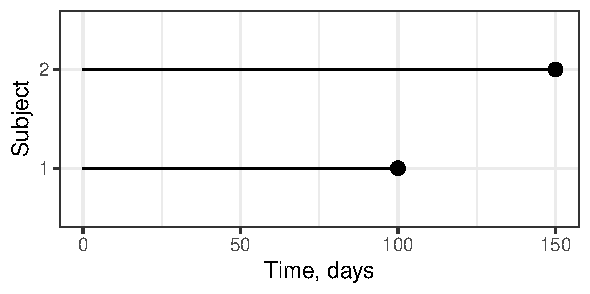
\includegraphics[width=0.6\textwidth]{../curve-cox/timeplot_1_light.pdf}
	\caption{
	An example of time to event data. Two subjects are followed from time 0. Subject 1 experiences the even at time 100. Subject 2 experiences the event at time 150.
	}
	\label{CoxExampleFull}
\end{figure}

Since subject 2 experienced the event later (i.e. ``survived'' for longer), the covariate pattern (e.g. antibody titre) of subject 2 would be considered by the model to be more ``protective'' than that of subject 1.

If subjects are not at risk of the event for all of their follow-up time (e.g. not exposed to the virus), then the total follow-up time may be misleading as illustrated in Figure \ref{CoxExamplePartial}. Taking the actual time at risk into account would lead to the opposite conclusion in this example --- it is subject 1 who is more ``protected'' since they were at risk for longer.

\begin{figure}[htp]
	\centering
	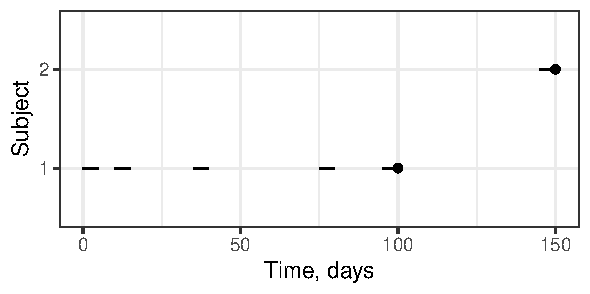
\includegraphics[width=0.6\textwidth]{../curve-cox/timeplot_2_light.pdf}
	\caption{
	An example of time to event data. Two subjects are followed from time 0. Subject 1 experiences the even at time 100. Subject 2 experiences the event at time 150. Subject 1 was at risk of the event for a total of 5 days. Subject 2 was at risk of the event for a total of 25 days.
	}
	\label{CoxExamplePartial}
\end{figure}

\pagebreak

In infection data, true time at risk is unobservable. If follow-up time is completely unrepresentative of true time at risk, the Cox model will not produce reliable results. However, if the total time of follow-up is assumed to be, on average, proportional to the total time at risk (e.g. subjects who are followed up for longer can be expected to have been exposed for longer) then the situation illustrated in Figure  \ref{CoxExamplePartial} will be ``averaged out'' and the model may still produce reliable results.

To investigate this, I simulated data. The model behind the simulations was

\begin{align*}
\begin{gathered}
T \sim \text{Exponential}(\text{rate} = \lambda) \\
h(t) = \lambda \\
\text{log}\lambda = -3 - 1.5 X_{\text{logtitre}}
\end{gathered}
\end{align*}

Where $T$ is the survival time, $h$ is the hazard and $X_{\text{logtitre}}$ is the true logtitre measurement simulated from $N(2, 2^2)$.

Each individual was assigned a proportion of time they were exposed to the virus. This proportion was generated from $\text{Beta}(10, 10\frac{1-m}{m})$ where $m$ is the expected proportion for the population. When $m$ was 1, the proportion assigned was always 1 to represent the ideal context of all follow-up time being time at risk. The maximum time of follow-up was set to 200 (days). If an individual's true survival time (a random number generated by $\text{Exponential}(\text{rate} = \text{exp}(-3 - 1.5 X_{\text{logtitre}}) )$ was at most 200 times their ``time at risk proportion'', then they were ``infected''. Otherwise, they were ``not infected''. 

Recorded time for each individual was 200 for everyone not infected (i.e. they were followed for the entire follow-up period and did not experience the event) and the true survival time divided by ``time at risk proportion'' for everyone infected (i.e. they were followed for that amount of time before experiencing the event).

I did 10,000 simulations with 10,000 observations in each at different values of the expected proportion of time at risk. I fit the Cox proportional hazards model to each simulated dataset. From 10,000 simulations at each value of the expected proportion at risk, I took the mean of the estimated coefficient (a measure of its expected value at that proportion) and its standard deviation (a measure of its expected standard error at that proportion and sample size). The results are summarised in Figure \ref{CoxSimResults}.

In the ideal case (proportion of time at risk set to 1) the estimate is unbiased and has the smallest error. As the proportion of time at risk decreases, bias is introduced while the error remains almost constant. When the proportion is small (less than 20\%), bias appears to decrease while error increases.

The maximum bias was less than 4\% away from the true value. The standard error increases notably only when the expected proportion at risk is very small (less than 10\%). This shows that under the assumption that the time of follow-up is proportional to time at risk, the Cox model can be expected to produce reliable results.

\pagebreak

\begin{figure}[htp]
	\centering
	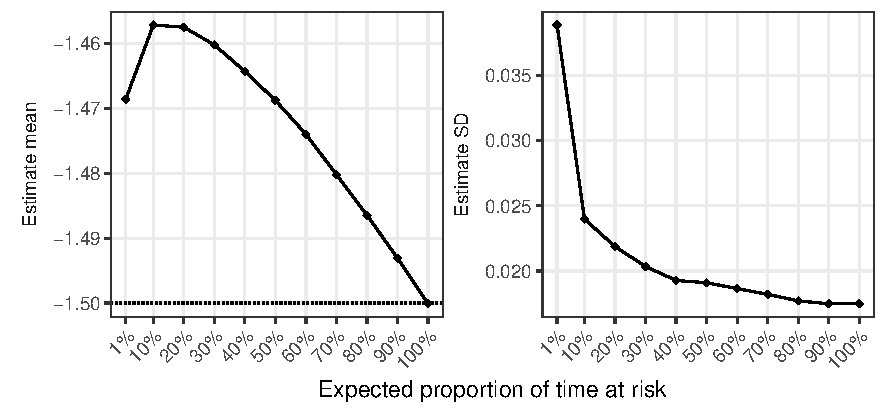
\includegraphics[width=1\textwidth]{../cox-tarprop-plot/risk.pdf}
	\caption{
	The results of time to event simulations. For each proportion of time at risk the mean of the estimated coefficient (left panel) is shown as well its standard deviation (right panel) obtained from 10,000 simulations. Points represent the values of expected proportion for which the simulations were performed. The dotted horizontal line is the true value of the estimated parameter.
	}
	\label{CoxSimResults}
\end{figure}

The assumption of time at risk being proportional to tome of follow-up is likely to hold when everyone in the sample is followed up through the period of similar disease activity. If the disease is seasonal, the start of follow-up can be set to the start of the season. For those who do not get infected, end of follow-up can then be the end of the season. For those who do get infected, end of follow-up can be the infection time assuming that infection grants immunity for the rest of the season. An illustration is in Figure \ref{CoxIdeal}.

The assumption will likely not hold if, with a seasonal disease, there are people in the sample whose follow-up starts before the season. An illustration is in Figure \ref{CoxNotIdeal}. For those with earlier follow-up start, their follow-up time will be large regardless of their titres (since they spend a proportion of that time not being at risk). This should make it seem like the titres have a smaller effect than they actually do thus biasing the estimate of titre effect towards the null.

To verify that having subjects in the sample whose follow-up starts prior to the season leads to bias towards the null, I did additional simulations with the same procedure as described above except subjects were randomly chosen to have had their follow-up started earlier. For those chosen, a uniform random number between 0 and 200 (days) was added to their recorded follow-up time. The proportion of time at risk was set to 1. How different proportions of the sample with earlier follow-up start affected the bias of the estimates is shown in Figure \ref{CoxSimLong}.

The estimate is unbiased when nobody in the sample has their follow-up started earlier than the start of the season. Bias towards the null increases rapidly even when only a small (10\%) proportion of the sample has its follow-up started prior to the season. For this reason, it would be advisable to record follow-up time in such a way so that true unobservable time at risk can be reasonably expected to be proportional to the recorded time of follow-up (i.e. the longer a subject is followed, the longer they are likely to have been at risk).

\pagebreak

\begin{figure}[htp]
	\centering
	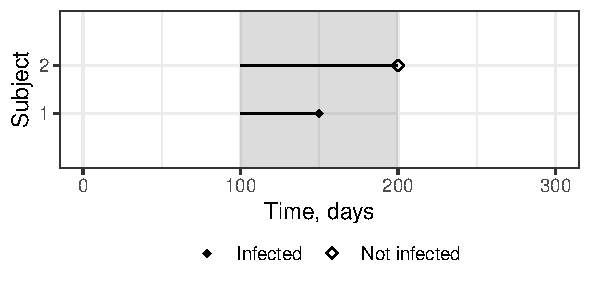
\includegraphics[width=0.59\textwidth]{../curve-cox/timeplot_3_light.pdf}
	\caption{
	An illustration of a pattern of follow-up where the assumption of true time at risk being proportional to time of follow-up is likely to hold. The shaded region marks the period of time when the disease is active. Both subject's follow-up starts at the beginning of the disease season (activity). Subject 1 gets infected at 150 days, their follow-up would end there assuming infection grants immunity (their total recorded time of follow-up would be 50 days). Subject 2 does not get infected through the season, their time of follow-up ends at the end of the season (their total recorded time of follow-up would be 100 days).
	}
	\label{CoxIdeal}
\end{figure}

\begin{figure}[htp]
	\centering
	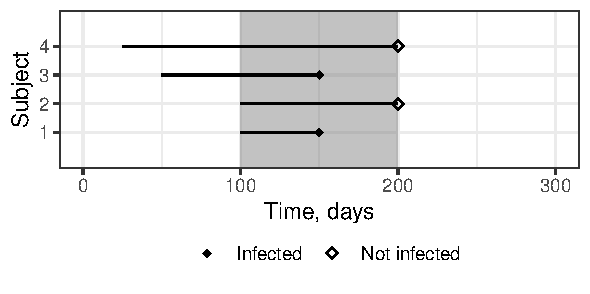
\includegraphics[width=0.59\textwidth]{../curve-cox/timeplot_4_light.pdf}
	\caption{
	An illustration of a pattern of follow-up where the assumption of true time at risk being proportional to time of follow-up is likely to not hold. The shaded region marks the period of time when the disease is active. Subject 1 gets infected at 150 days, their follow-up would end there assuming infection grants immunity (their total recorded time of follow-up would be 50 days). Subject 2 does not get infected through the season, their time of follow-up ends at the end of the season (their total recorded time of follow-up would be 100 days). Subjects 3 (recorded follow up of 100 days) and 4 (recorded follow-up of 175 days) had follow-up started prior to season onset.
	}
	\label{CoxNotIdeal}
\end{figure}

\pagebreak

\begin{figure}[htp]
	\centering
	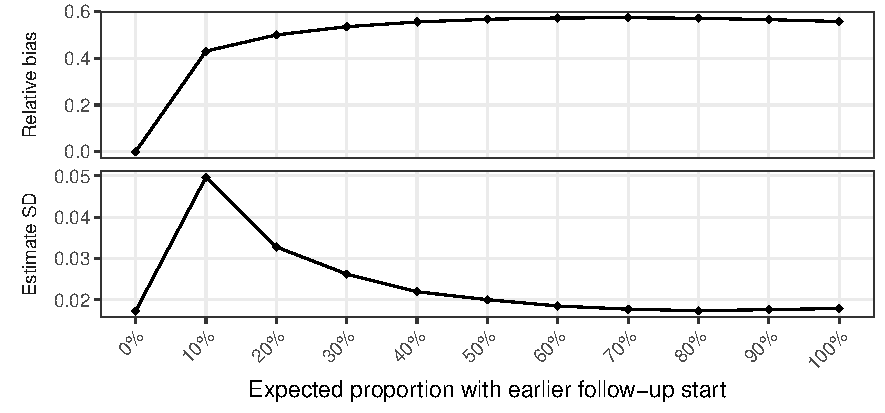
\includegraphics[width=1\textwidth]{../cox-tarprop-plot/long.pdf}
	\caption{
	The results of time to event simulations. For each proportion of the sample with earlier follow-up start, the mean of the estimated coefficient (left panel) is shown as well as the standard deviation of that coefficient (right panel) from 10,000 simulations. Points represent the values of expected proportion for which the simulations were performed. The dotted horizontal line is the true value of the estimated parameter.
	}
	\label{CoxSimLong}
\end{figure}

\pagebreak
%
\section{Logistic regression}

This model assumes that the probability of outcome follows a logistic curve from 1 (at low covariate values assuming a protective covariate) to 0 (at high covariate values). If there is only one covariate which is the antibody titre measurement, then the model is

\begin{align*}
\begin{gathered}
P(Y=1) = \frac{\text{exp}(\beta_0 + \beta_T X_{\text{logtitre}})}{1 + \text{exp}(\beta_0 + \beta_T X_{\text{logtitre}})}
\end{gathered}
\end{align*}

A potentially large problem with the application of this model to antibody data is that low antibody titres do not necessarily guarantee infection (which is one of the model's assumptions). As an example, this assumption is not justified in the Hanam data as shown in Figure \ref{HanamCounts}. In both the general and the exposed populations, less than half the subjects with the titres below detectable levels (recorded as 5) were infected.

\begin{figure}[htp]
	\centering
	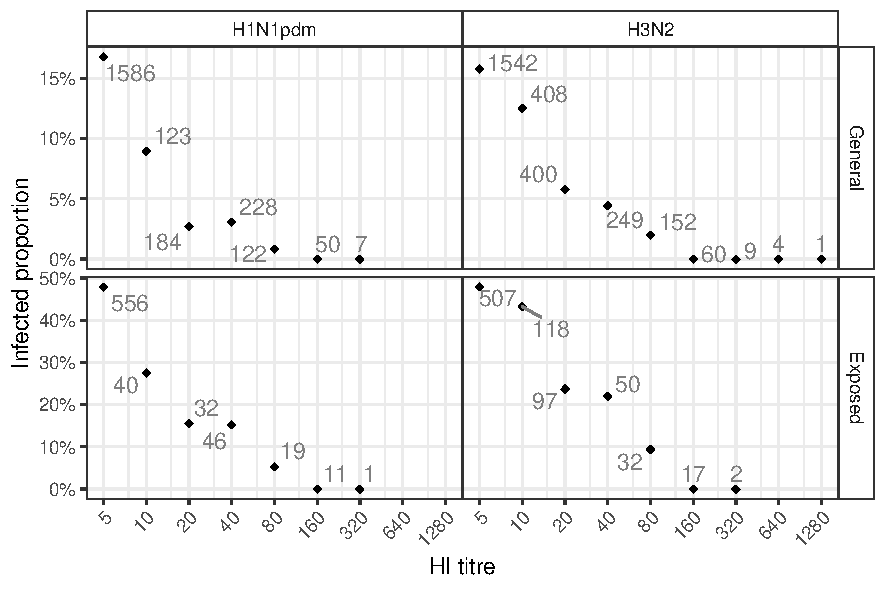
\includegraphics[width=0.9\textwidth]{../data-plot/hanam-hi-summ-light.pdf}
	\caption{
	Hanam cohort data. Subjects were grouped by virus and measured HI titre. Numbers next to points are the total number of observations in the corresponding group. The top row is all observations. The bottom row are the observations from households with at least one infection in a given season. The left column is observations for the H1N1pdm virus, the right row --- for H3N2 virus.
	}
	\label{HanamCounts}
\end{figure}

If the assumption of the baseline probability being 1 is not satisfied, the fitted probability curve will be flatter than the real one thereby misrepresenting the true probability of infection across the titre range. An illustration is in Figure \ref{LogisticFit}.

\pagebreak

\begin{figure}[htp]
	\centering
	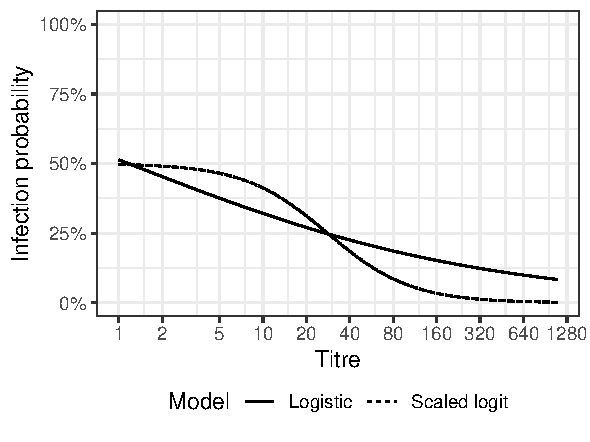
\includegraphics[width=0.6\textwidth]{../logistic-plot/lrex.pdf}
	\caption{
	An illustration of a bad fit of the logistic model. The dotted line (overlaps the dashed line) is the true probability curve $0.5\frac{\text{exp}(5 - 1.5 X_{\text{logtitre}})}{1 + \text{exp}(5 - 1.5 X_{\text{logtitre}})}$. The solid line is the expected fitted probability curve from standard logistic regression. The dashed line (overlaps the dotted line) is the expected fitted probability curve from scaled logistic regression. The expected curves was obtained from 10,000 simulations each with 10,000 observations simulated from the true curve. The models were fitted to each simulated dataset and the means of the regression estimates were taken from all simulations.
	}
	\label{LogisticFit}
\end{figure}

The potential bias in the estimates coming from fitting the logistic model is the reason why the logistic model is unreliable whenever the assumption of the baseline risk of 1 cannot be justified.

\pagebreak
%
\section{Scaled logistic regression}

This model is the same as logistic regression except that it estimates the baseline probability of outcome (i.e. the probability at low covariate values assuming a protective covariate) as opposed to assuming that it is equal to 1. If there is only one covariate which is the antibody titre measurement then the model is

\begin{align*}
\begin{gathered}
P(Y=1) = \frac{\lambda}{1 + \text{exp}(\beta_0 + \beta_T X_{\text{logtitre}})}
\end{gathered}
\end{align*}

Note that with the above parameterisation, the $\beta$ parameters are negated relative to logistic regression.

The model still assumes that low probability bound is 0 (i.e. that high titres guarantee immunity in a univariate model). This assumption is justified if there is a reasonable number of people in the sample who have high titres and none (or very few) of whom get infected. In the Hanam data (Figure \ref{HanamCounts}), there is a total of 131 observations with titres above 160. None of those subjects got infected in the corresponding season justifying the assumption that high titres guarantee immunity.

Compared to logistic regression, the scaled logit model requires a larger sample size. This is because the scaled logit model attempts to use the same amount of information to estimate one more parameter. This leads to larger standard errors and potential convergence problems. Figures \ref{SclrSE} and \ref{SclrConv} summarise 10,000 simulation results from the model $\frac{0.5}{\text{exp}(-5 + 1.5 X_{\text{logtitre}})}$ with $X_{\text{logtitre}}$ simulated from $N(2, 2^2)$. Logistic and scaled logit models were fit using maximum likelihood estimation. 

Standard errors of the $\beta$ regression estimates ($\beta_0$ being the intercept and $\beta_T$ being $X_{\text{logtitre}}$ coefficient) were consistently higher with the scaled logit model. In order to reliably converge (under the chosen true parameter values) the scaled logit model required the sample size to be over 500. The standard logistic model always converged.

\pagebreak

\begin{figure}[htp]
	\centering
	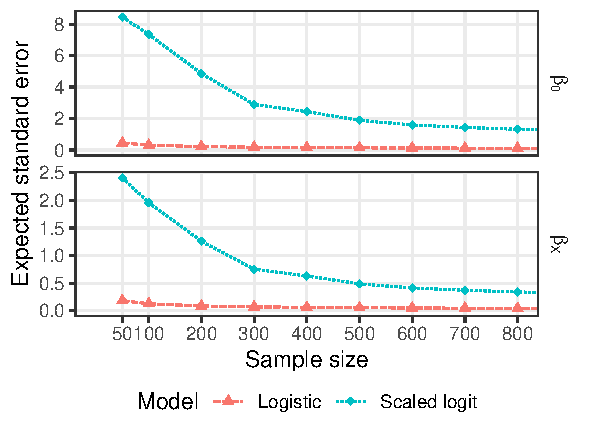
\includegraphics[width=0.69\textwidth]{../logistic-plot/vary_nsam_se.pdf}
	\caption{
	Simulation results of fitting the standard logistic and the scaled logit models to the same simulated datasets. 10,000 datasets were simulated. Shown is the mean standard deviation (estimate of the expected standard error) of the $\beta$ regression estimates from the standard logistic (the solid line) and the scaled logit (the dashed line). Points indicate parameter values at which the simulations were performed.
	}
	\label{SclrSE}
\end{figure}

\begin{figure}[H]
	\centering
	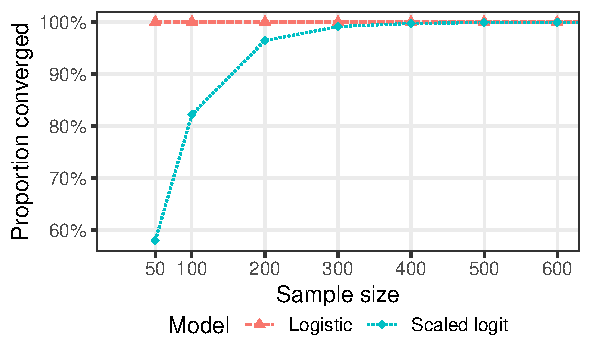
\includegraphics[width=0.69\textwidth]{../logistic-plot/vary_nsam.pdf}
	\caption{
	Simulation results of fitting the standard logistic and the scaled logit models to the same simulated datasets. 10,000 datasets were simulated. Shown is the proportion of successful attempts to fit the standard logistic (the solid line) and the scaled logit (the dashed line) model. Points indicate parameter values at which the simulations were performed.
	}
	\label{SclrConv}
\end{figure}

\pagebreak
%
\section{Hanam application}

This section shows an application of the scaled logit model to the Hanam cohort which is plotted in Figure \ref{HanamCounts}. For this cohort, the Cox model is inapplicable due to absence of reliable data on disease activity. The standard logistic model is inappropriate due to unjustified assumption of baseline of 1.

\subsection{Scaled logit fit}

The scaled logit model was fit in a Bayesian way to better handle missing data and censored titre measurements. The full specification is

\begin{align*}
\begin{gathered}
Y_i \sim \text{Bernoulli}(p_i) \\
p_i = \frac{\lambda}{1 + \text{exp}(\beta_0 + \beta_T T_i)} \\
T_i \sim N(\mu, \sigma^2) \ \text{truncated}(L_{i}, H_{i}) \\
\mu \sim N(2, 2^2) \quad \sigma \sim \text{Exponential}(\text{rate} = 0.1) \\
\lambda \sim \text{Uniform}(0, 1) \\
\beta_0 \sim N(-15, 10^2) \quad \beta_T \sim N(5, 5^2)
\end{gathered}
\end{align*}

Where $i$ is observation index, $Y_i$ is infection status (0 --- infected (both symptomatic and asymptomatic), 1 --- not infected), $T_i$ is true log HI titre, $L_i$ is the low bound of observed HI interval (e.g. for observation of 20 this is log(20)), $H_i$ is the high bound of observed HI interval (e.g. for observation of 20 this is log(40)).

The prior distributions for the mean and standard deviation of log HI titres were chosen to be broad but still somewhat reflect the expected distribution in the general population --- mean high enough to allow a fair proportion (>20\%) to have titres above detectable level (log(10)) and standard deviation low enough to not result in titres above highest detectable level (log(1280)) to be more prevalent than titres between log(640) and log(1280).

The prior distribution for the baseline risk parameter $\lambda$ gives equal probability to all of its possible values. The prior distributions for the logistic curve parameters $\beta_0$ and $\beta_T$ was chosen to be spread around all of their plausible values --- $\beta_0$ is likely below 0 (otherwise the probability of infection would be close to 0 and not change across the observed titre range) and not too low (e.g. a value below -30 would result in the probability of infection being equal to $\lambda$ and not changing across the observed titre range); while $\beta_T$ is likely above 0 (since titres are protective) but not too high since it would result in a very steep curve (e.g. a titre of 20 may have the expected infection probability of $\lambda$ while a titre of 40 has the expected infection probability of 0).

The fitted infection curve is shown in Figure \ref{SclrBayesInf}. The fitted protection curve is shown in Figure \ref{SclrBayesProt}.

\begin{figure}[htp]
	\centering
	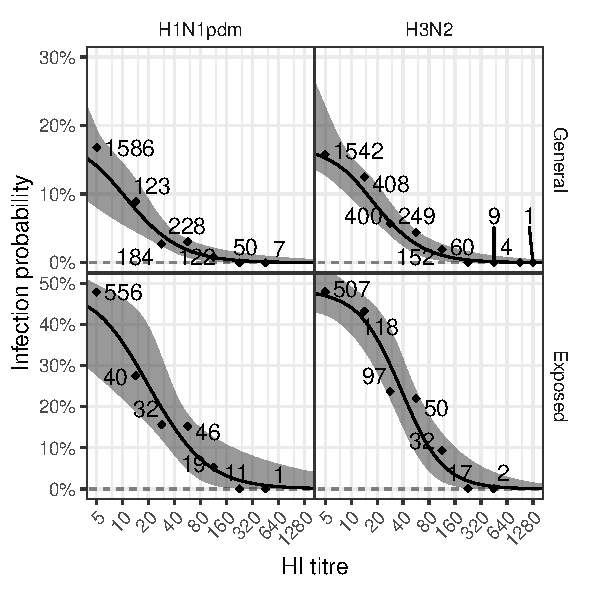
\includegraphics[width=0.8\textwidth]{../fit-sclr-bayesian-plot/hanam-hi-inf.pdf}
	\caption{
	Fitted infection curve and credible interval from the scaled logit model Bayesian fit to Hanam data (also shown in Figure \ref{HanamCounts}). The solid line is the median of the posterior distribution. The shaded region is the 95\% credible interval. The dashed line is the prior distribution, i.e. the bounds of the shaded region that would have been obtained if the data contained no information to estimate model parameters. The upper bound is above 90\% and therefore not visible. The points are the infected proportions at the corresponding titre measurements. The numbers next to the points are the total sample size of the corresponding groups. Note that the titre measurements were shifted to midpoints of the corresponding intervals to better represent average underlying titres, e.g. the measurement of 20 was shifted to the log-scale midpoint between 20 and 40 (except the measurement of 5 which represents undetectable titres and the measurement of 1280 which represents titres above the highest detectable level).
	}
	\label{SclrBayesInf}
\end{figure}

\pagebreak

\begin{figure}[htp]
	\centering
	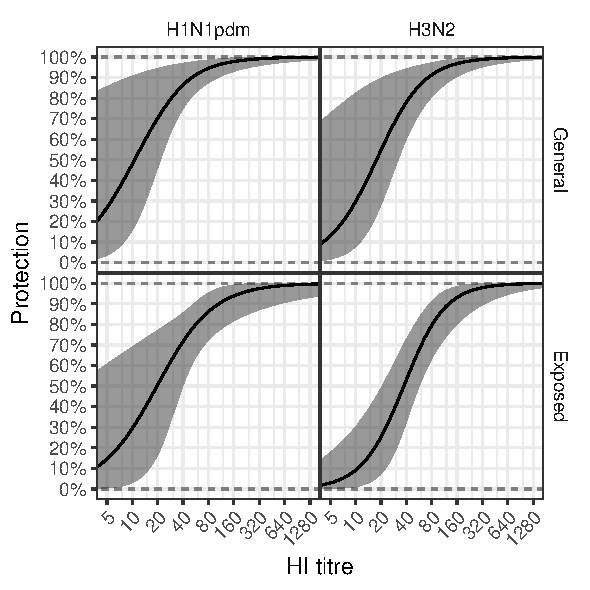
\includegraphics[width=0.8\textwidth]{../fit-sclr-bayesian-plot/hanam-hi-prot.pdf}
	\caption{
	Fitted protection curve and credible interval from the scaled logit model Bayesian fit to Hanam data (also shown in Figure \ref{HanamCounts}). The solid line is the median of the posterior distribution. The shaded region is the 95\% credible interval. The dashed line is the prior distribution, i.e. the bounds of the shaded region that would have been obtained if the data contained no information to estimate model parameters.
	}
	\label{SclrBayesProt}
\end{figure}

Limiting the sample to just those exposed to the virus (at least one household infection in a season) improved the precision of the estimates. Despite a fairly large sample, reasonably precise estimates of 50\% protection can only be obtained for the H3N2 virus (inferring from the model fitted to the exposed subset). The general lack of precision in the estimates is likely due the number of parameters in the model (3 parameters with 1 covariate) and the censored nature of HI titre measurements, particularly the fact that any titre below 10 is undetectable which means that it is impossible to distinguish between many of the observations (e.g. some subjects with undetectable titres may have had a true titre of 9 while others --- of 2, but both were recorded as 5) which makes it harder to estimate the baseline probability (as seen in the credible bounds increasing at small (<10) titres).

\pagebreak
%
\subsection{Comparison to standard logistic fit}

As mentioned before, the standard logistic model is inappropriate due to unsatisfied assumption of baseline of 1. It was fit to the same Hanam data using maximum likelihood with no accounting for censored titres (observations of 5 (below detectable) and 1280 (above detectable) were unchanged, all other observations were moved to the midpoint of the corresponding censored interval on a log scale). The fitted infection curve is in Figure \ref{lr-inf}.
-ba
\begin{figure}[htp]
	\centering
	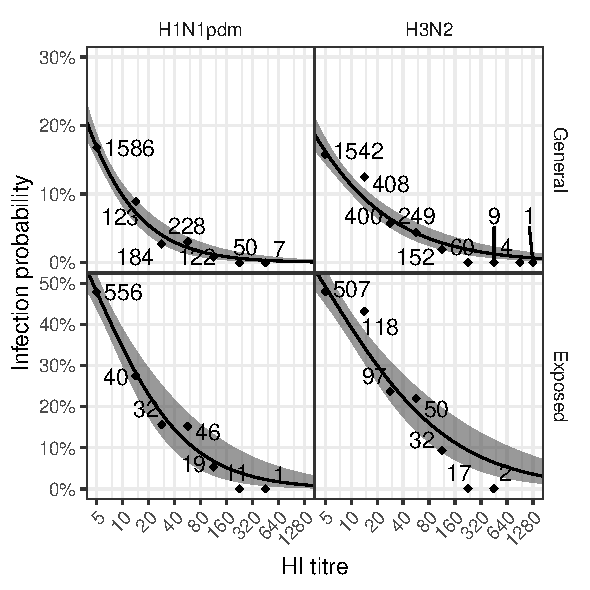
\includegraphics[width=0.8\textwidth]{../fit-logistic-plot/hanam-hi-inf.pdf}
	\caption{
	Fitted infection curves and confidence intervals from the standard logistic model fit to Hanam data (also shown in Figure \ref{HanamCounts}) using maximum likelihood with no accounting of censored titres (observations of 5 (below detectable) and 1280 (above detectable) were unchanged, all other observations were moved to the midpoints of the corresponding censored intervals on a log scale). The points are the infected proportions at the corresponding modified titre measurements (i.e. interval midpoints). The solid line is the point estimates. The shaded region is the 95\% confidence interval. The numbers next to the points are the total sample size of the corresponding groups.
	}
	\label{lr-inf}
\end{figure}

\pagebreak

While the infection curves appear to fit the data well, it is problematic to generate a protection curve from these results. There are two options for the protection curve. One is to use the same procedure as was used in the scaled logit fit --- divide the fitted infection probabilities by the baseline (here assumed to be 1, so the fitted values would not change) and subtract the resulting relative-to-baseline infection probabilities from 1. The protection curves resulting from this procedure are in Figure \ref{lr-prot-abs}.

\begin{figure}[htp]
	\centering
	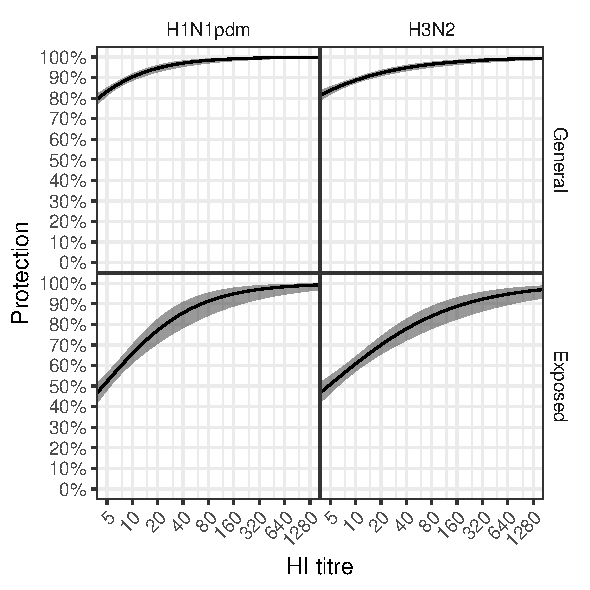
\includegraphics[width=0.8\textwidth]{../fit-logistic-plot/hanam-hi-prot.pdf}
	\caption{
	Fitted protection curves and confidence intervals from the standard logistic model fit to Hanam data (also shown in Figure \ref{HanamCounts}) using maximum likelihood with no accounting of censored titres (observations of 5 (below detectable) and 1280 (above detectable) were unchanged, all other observations were moved to the midpoints of the corresponding censored intervals on a log scale). The solid line is the point estimates. The shaded region is the 95\% confidence interval.
	}
	\label{lr-prot-abs}
\end{figure}

The other option for generating a protection curve is to calculate the fitted probability of infection at a give titre and divide that by the fitted probability of infection at the titre of 5 (or any other) thereby generating a curve that shows relative-to-5 infection probabilities (as opposed to relative-to-baseline). Subtracting these relative-to-5 infection probabilities from 1 generates curves shown in Figure \ref{lr-prot-rel}

\pagebreak

\begin{figure}[htp]
	\centering
	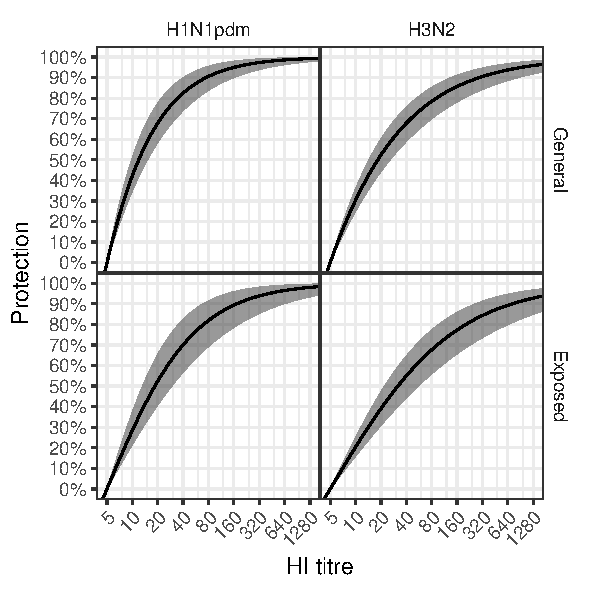
\includegraphics[width=0.8\textwidth]{../fit-logistic-boot-plot/hanam-hi-prot-rel.pdf}
	\caption{
	Fitted relative-to-5 protection curves and confidence intervals from the standard logistic model fit to Hanam data (also shown in Figure \ref{HanamCounts}) using maximum likelihood with no accounting of censored titres (observations of 5 (below detectable) and 1280 (above detectable) were unchanged, all other observations were moved to the midpoints of the corresponding censored intervals on a log scale). The solid line is the point estimates. The shaded region is the 95\% confidence interval.
	}
	\label{lr-prot-rel}
\end{figure}

While the relative-to-5 protection curves (Figure \ref{lr-prot-rel}) appear more plausible than the relative-to-baseline protection curves (Figure \ref{lr-prot-abs}), both result from fitting a model with an unsatisfied assumption and neither method of generating protection curves from logistic regression model fit will reliably produce accurate results.

The relative-to-5 curve (Figure \ref{lr-prot-rel}) presents an additional problem. The curve shows how much ``better'' different titres are at protecting against infection than the titre of 5 (or some other threshold). There is nothing inherently special about this threshold of 5 and its choice is arbitrary. The curves may look substantially different if a different threshold (e.g. 10 or 1) is chosen.

\pagebreak
%
\section{Kiddyvax application}

The data for this study includes post-vaccination HI titres of subjects who were followed up for a year for flu infection. The infection status was determined by PCR which was done for everyone who experienced symptoms. This data is shown in Figure \ref{fig:kiddyvax-main-titre}.

\begin{figure}[htp]
	\centering
	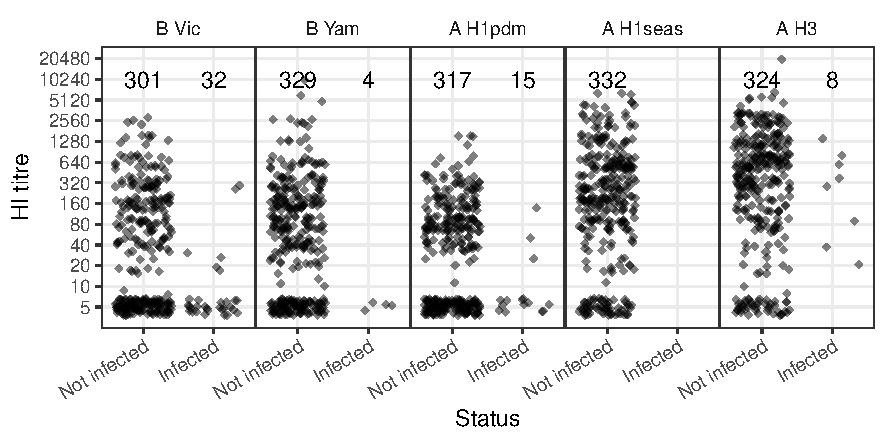
\includegraphics[width=1\textwidth]{../data-plot/kiddyvax-main-titre.pdf}
	\caption{
	Kiddyvax study data. Post-vaccination titres are shown for those who got infected (PCR-confirmed symptomatic infection) over the course of the study and those who did not. Panels correspond to the five tested viruses.
	}
	\label{fig:kiddyvax-main-titre}
\end{figure}

Analyses were done on the data for B Vic and A(H1pdm) viruses in the same way as for the Hanam data with the addition of the Cox proportional hazards model.

\pagebreak
%
\subsection{Scaled logit fit}

The same model was fit in the same way using the same prior distributions as for the Hanam data. The protection curves are in Figure \ref{fig:kiddyvaxmain-prot-bayes-sclr}.

\begin{figure}[htp]
	\centering
	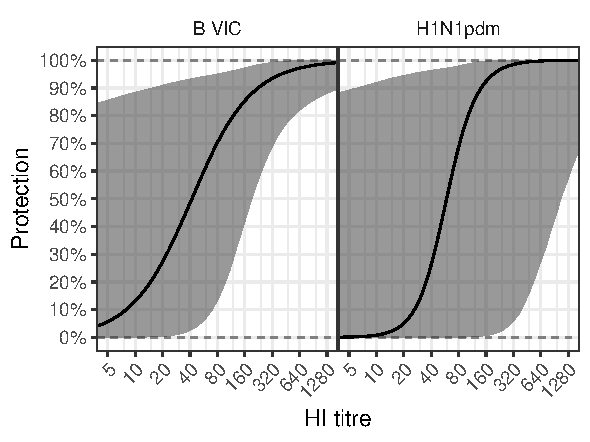
\includegraphics[width=0.8\textwidth]{../fit-sclr-bayesian-plot/kiddyvaxmain-prot.pdf}
	\caption{
Fitted infection curve and credible interval from the scaled logit model Bayesian fit to subsets of kiddyvax data (shown in Figure \ref{fig:kiddyvax-main-titre}). The solid line is the median of the posterior distribution. The shaded region is the 95\% credible interval. The dashed line is the prior distribution, i.e. the bounds of the shaded region that would have been obtained if the data contained no information to estimate model parameters.
	}
	\label{fig:kiddyvaxmain-prot-bayes-sclr}
\end{figure}

The credible intervals are very broad due to the fact there are very few infections the the sample.

\pagebreak
%
\subsection{Standard logistic fit}

The relative protection curves are in Figure \ref{fig:kiddyvaxmain-prot-rel-lr-boot}.

\begin{figure}[htp]
	\centering
	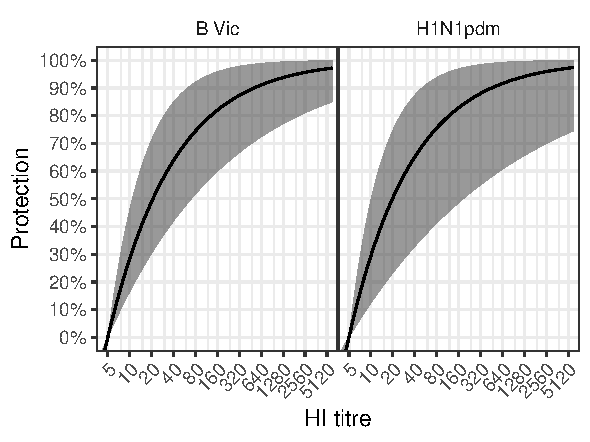
\includegraphics[width=0.8\textwidth]{../fit-logistic-boot-plot/kiddyvaxmain-prot-rel.pdf}
	\caption{
	Fitted relative-to-5 protection curves and confidence intervals from the standard logistic model fit to kiddyvax data (shown in Figure \ref{fig:kiddyvax-main-titre}) using maximum likelihood with no accounting of censored titres (observations of 5 (below detectable) were unchanged, all other observations were moved to the midpoints of the corresponding censored intervals on a log scale). The solid line is the point estimates. The shaded region is the 95\% confidence interval.
	}
	\label{fig:kiddyvaxmain-prot-rel-lr-boot}
\end{figure}

The same considerations regarding the unjustified assumption of baseline risk of 1 apply here as they did with Hanam (Figure \ref{fig:kiddyvax-main-titre} shows many uninfected subjects with undetectable titres).

\subsection{Cox proportional hazards fit}

For those who got infected, the time at risk was taken to be the time from start of follow-up to infection. For those who did not get infected the time at risk was take to be the time from start of follow-up to end of follow-up.

The model was

\begin{align*}
\begin{gathered}
h(t) = h_0\text{exp}(\beta_T X_{\text{logtitre}})
\end{gathered}
\end{align*}

where $h$ is the hazard function and $X_{\text{logtitre}}$ is the post-vaccination titre measurement on the log scale.

The resulting protection curves (relative to the titre of 5) are in Figure \ref{fig:kiddyvaxmain-cox}.

\begin{figure}[htp]
	\centering
	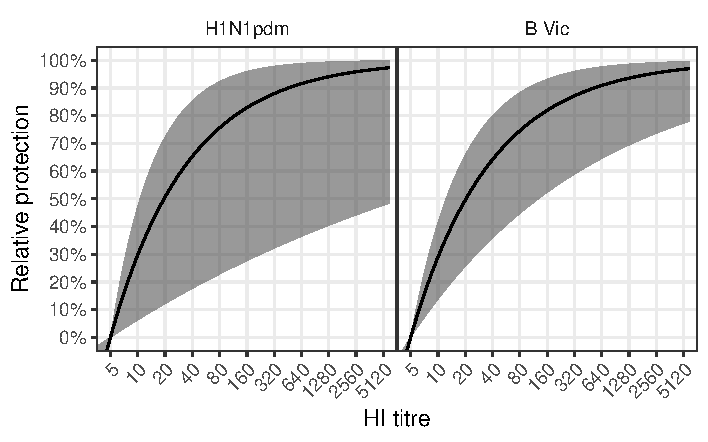
\includegraphics[width=0.8\textwidth]{../fit-cox-plot/kiddyvaxmain.pdf}
	\caption{
	Fitted relative-to-5 protection curves and confidence intervals from the Cox proportional hazards model fit to kiddyvax data (shown in Figure \ref{fig:kiddyvax-main-titre}) with no accounting of censored titres (observations of 5 (below detectable) were unchanged, all other observations were moved to the midpoints of the corresponding censored intervals on a log scale). The solid line is the point estimates. The shaded region is the 95\% confidence interval.
	}
	\label{fig:kiddyvaxmain-cox}
\end{figure}

\pagebreak
%
\section{Conclusion}

\begin{table}[htp]
\centering
\caption{Summary of the three considered models in terms of their application to antibody data}
\begin{tabular}{cp{25em}}
\toprule
Model & Potential problem \\
\midrule
Cox PH & Biased if follow-up time is not proportional to time at risk for everyone in the sample \\
Logistic & Biased if low antibody titres do not guarantee immunity \\
Scaled logit & Requires a large sample size. \\
\bottomrule
\end{tabular}
\end{table}

In presence of good time to event data where every subject's follow-up time is at least proportional to their time at risk, the Cox model will likely perform best out the the three due to it having the least number of parameters allowing for more precise estimates. In absence of such data, logistic regression may be applicable if the assumption of everyone being infected at low antibody titres can be justified. If this assumption cannot be justified, the scaled logit model can be applied but the sample needs to be fairly large (>500) in order to obtain useful estimates.

\end{document}
